\documentclass[french,english,12pt]{exam}

\printanswers

\usepackage{../../latex/macro_mealor}
\usepackage[utf8]{inputenc}
\usepackage[T1]{fontenc} % accents codés dans la fonte
%\usepackage{layout}
\usepackage{a4wide}
%\usepackage[french]{babel}
\usepackage{hyperref}

\usepackage{graphicx}
\usepackage{caption}

\usepackage{newpxtext,newpxmath}
\usepackage{siunitx}

%\setlength{\hoffset}{0pt}
%\setlength{\oddsidemargin}{-1cm}   % Marge gauche sur pages impaires
%\setlength{\evensidemargin}{-1cm}   % Marge gauche sur pages paires
%\setlength{\marginparwidth}{0cm}   % Largeur de note dans la marge
%\setlength{\textwidth}{16cm}   % Largeur de la zone de texte (17cm)
\setlength{\voffset}{0pt}   % Bon pour DOS
\setlength{\marginparsep}{0pt}   % Séparation de la marge
\setlength{\topmargin}{0cm}   % Pas de marge en haut
\setlength{\headheight}{0cm}   % Haut de page
\setlength{\headsep}{0cm}   % Entre le haut de page et le texte
%\setlength{\footskip}{1cm}   % Bas de page + séparation
%\setlength{\textheight}{25.5cm}   % Hauteur de la zone de texte (25cm)

\usepackage{indentfirst}


\newcommand{\classurl}{\url{1}}
% #1 numéro de la feuille
% #2 titre de la feuille
\newcommand{\titre}[3] {%\textit{
  \begin{center}\textbf{\textsc{MEALOR II}}\\ \textit{Mécanique de l'endommagement et approche locale de la rupture}%\let\thefootnote\relax\footnotetext{\classurl} 
  \end{center}
 
  \noindent TD n\textdegree #1 \hfill  August 2023\\[-0.3cm]
  \rule{\linewidth}{.3mm}
  \vspace*{0.5pt}
  \begin{center}
    {
      \Large \bfseries { #2}
    }\\
    \vspace*{0.5cm}
	\large #3
    \vspace*{0.5cm}
  \end{center}
}

\usepackage{xcolor}
\definecolor{Blue}{RGB}{0,68,170}
\SolutionEmphasis{\normalfont\color{Blue}}
\DeclareCaptionFont{blue}{\color{Blue}}

\newenvironment{objectifs}
    {\itshape\underline{Objectifs:}\begin{itemize}
    }
    { \itshape
    \end{itemize}
    }
    
\newcounter{Rfig}
\newenvironment{R_figure}
   {\begin{minipage}{\linewidth}\begin{center}\vspace{0.5mm}\stepcounter{Rfig}\addtocounter{figure}{-1}\renewcommand\thefigure{R-\arabic{Rfig}}
   \captionsetup{font=blue}}
   {\end{center}\vspace{0.5mm}\end{minipage}}
   
    
\newcounter{Rtab}
\newenvironment{R_table}
   {\begin{minipage}{\linewidth}\begin{center}\vspace{0.5mm}\stepcounter{Rtab}\addtocounter{table}{-1}\renewcommand\thetable{R-\arabic{Rtab}}
   \captionsetup{font=blue}
}
   {\end{center}\vspace{0.5mm}\end{minipage}}
   
      
\graphicspath{{./pic/}}
\usepackage{float}

\begin{document}
\thispagestyle{empty}
\titre{3}{Rupture ductile : homogénéisation de matériaux poreux}{Jérémy Hure, Djimédo Kondo, Jérémy Bleyer}

\begin{objectifs}
\item obtenir un critère de plasticité pour matériaux poreux dans le cadre de la modélisation de la rupture ductile
\item discuter des effets d'anisotropie
\end{objectifs}

 Le point de départ est de considérer le \textbf{critère de plasticité de von Mises} qui s'écrit:
\begin{equation}
  \phi\left( \td{\sigma}   \right) =  \sigma_{eq} - \sigma_0 \leq 0 \hspace{2cm} \sigma_{eq} = \sqrt{\frac{3}{2} \td{s} \cdot \td{s}} \ \ \ \ \mathrm{avec} \ \ \ \ \td{s} = \tsigma - \frac{1}{3} \mathrm{tr}\tsigma \td{I}
  \label{eq1}
\end{equation}
La déformation plastique se produit quand le critère est atteint, \textit{i.e.}, $\phi = 0$. Dans la suite, l'écrouissage n'est pas pris en compte ($\sigma_0 = C^{ste}$) et l'élasticité est ignorée, ce qui correspond à un matériau dit rigide parfaitement plastique.
%Le tenseur $\tq{A}$ contient les informations concernant l'anisotropie du matériau, et $\tsigma$ correspond au tenseur des contraintes de Cauchy. En notation de Voigt, ces tenseurs sont représentés par les matrices suivantes dans les axes d'orthotropies:
%\begin{equation}
%  \tsigma = \begin{pmatrix}
%    \sigma_{11} \\
%    \sigma_{22} \\
%    \sigma_{33} \\
%    \sigma_{12} \\
%    \sigma_{13} \\
%    \sigma_{23} \\
%  \end{pmatrix} \hspace{2cm}
%  \tq{A} = \begin{pmatrix}
%    F + H & -F & -H & 0 & 0 & 0 \\
%    -F & G+ F & -G & 0 & 0 & 0 \\
%    -H & -G & G+H & 0 & 0 & 0 \\
%    0 & 0 & 0 & L & 0 & 0 \\
%    0 & 0 & 0 & 0 & M & 0 \\
%    0 & 0 & 0 & 0 & 0 & N \\
%    \end{pmatrix}
%\end{equation}
%Pour $F = G = H = 1/2$ et $L = M = N = 3/2$, le critère de Hill correspond au critère de von Mises.
La loi d'écoulement plastique associée permet d'obtenir le taux de déformation plastique:
\begin{equation}
  \td{d} = d_{eq} \frac{3 \td{s}}{2 \sigma_0}  \hspace{2cm} d_{eq} = \sqrt{\frac{2}{3}\td{d} \cdot \td{d} }
  \label{eq200}
\end{equation}
%où les paramètres du tenseur $\tq{B}$ sont reliés à ceux de $\tq{A}$ par les relations donnés en Annexe.\\
%\begin{itemize}
%  \item[$\bullet$] Quels paramètres est-il possible d'obtenir à partir des résultats expérimentaux ?\\
%\end{itemize}
\noindent
Afin d'étendre ce critère à la présence d'une porosité, la géométrie présentée sur la Fig.~1 est considérée, à savoir un cylindre creux de hauteur $L$, de rayons intérieur $a$ et extérieur $b$. La porosité, définie comme le rapport entre le volume de la cavité et le volume total est noté $f = (a/b)^2$.
\begin{figure}[H]
  \centering
  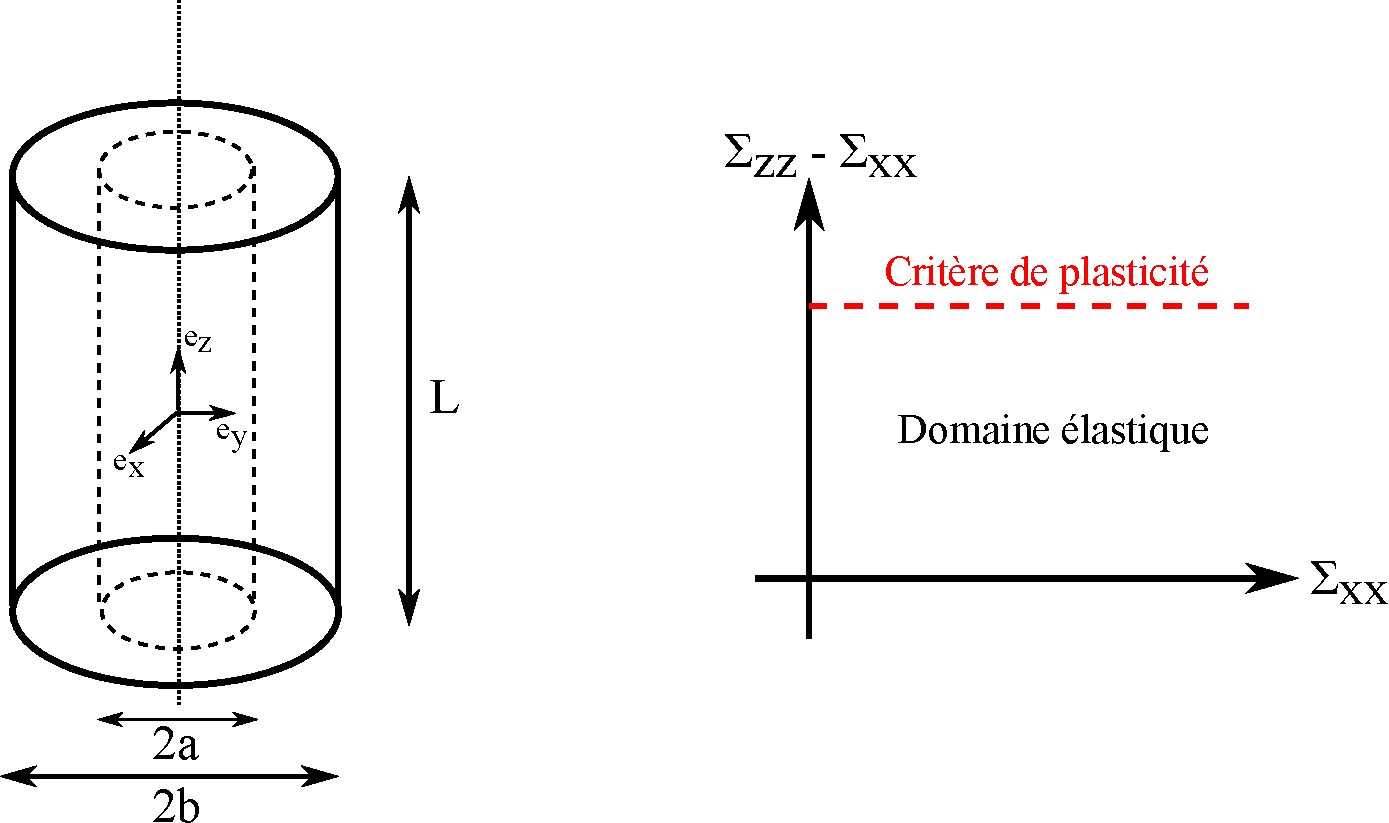
\includegraphics[height = 7cm]{homoMEALOR.pdf}
\caption{Géométrie considérée et critère de plasticité de la matrice}
\label{fig1}
\end{figure}

\begin{itemize}
\item[$\bullet$] Quel matériau peut être représenté par cette géométrie ? Dans le cas de chargement axisymétrique, montrer que le critère de plasticité de von Mises de la matrice entourant la cavité correspond à la Fig.~\ref{fig1}.\\
\end{itemize}
\noindent
%L'anisotropie considérée est un cas particulier de celle de Hill: le matériau est supposée isotrope dans le plan perpendiculaire à l'axe du cylindre (isotropie transerse), l'axe dy cylindre correspondant à l'axe d'orthotropie du matériau.\\

%\begin{itemize}
%  \item[$\bullet$] Quelles relations existent entre les paramètres de la matrice $\tq{A}$ dans le cas de l'isotropie transverse ?\\
%\end{itemize}

\noindent
La contrainte et le taux de déformation (plastique) macroscopique sont définis à l'échelle du cylindre par les relations suivantes:
\begin{equation}
  \tSigma = \frac{1}{V} \int_V \tsigma dV
\end{equation}
\begin{equation}
  \td{D} = \frac{1}{V} \int_V \td{d} \, dV = \frac{1}{2V} \int_{\partial V} \left(\td{v} \otimes \td{n} + \td{n} \otimes \td{v}     \right) dS
\end{equation}

\noindent
avec $\td{v}$ le champ de vitesse et $\td{n}$ la normale à la surface extérieure.\\

\noindent
Nous cherchons à obtenir le critère de plasticité du cylindre, c'est-à-dire l'équivalent de l'Eq.~\ref{eq1} pour les grandeurs macroscopiques $\tSigma$ et $\td{D}$. Pour cela, la théorie de l'analyse limite est utilisée. En pratique, celle-ci consiste à postuler un champ de vitesse $\td{v}$ admissible (dans un sens qui sera détaillé dans la suite), et à calculer la dissipation plastique associée:
\begin{equation}
  \Pi = \frac{1}{V} \int_V \sigma_0 d_{eq}(\td{v}) \,dV
  \label{eq3}
\end{equation}
\noindent
Sous certaines conditions (qui là-encore seront détaillées dans la suite), cette dissipation plastique permet d'évaluer la contrainte maximale admissible, c'est-à-dire le critère de plasticité, par les relations suivantes:
\begin{equation}
  \tSigma \cdot \td{D} \leq \Pi \hspace{2cm} \tSigma \leq \frac{\partial \Pi}{\partial \td{D}}
  \label{eq2}
\end{equation}

\noindent
Afin d'obtenir une estimation du critère de plasticité, la première étape consiste donc à choisir un champ de vitesse pris sous la forme:
\begin{equation}
  \td{v} = v_r(r) \td{e}_r + v_z(z) \td{e}_z 
\end{equation}

\begin{itemize}
\item[$\bullet$] En imposant que le champ de vitesse soit incompressible ($\mathrm{tr}\td{d} = 0$), montrer que celui-ci est de la forme:\\
\begin{equation}
  \td{v} = \left( \frac{B}{r} -  \frac{A}{2}r \right)  \td{e}_r +  A z \td{e}_z 
\end{equation}
\end{itemize}

\begin{itemize}
\item[$\bullet$] Comment s'écrit le taux de déformation macroscopique $\td{D}$ ? \\
\end{itemize}
  
\noindent
Ce champ de vitesse est \textbf{cinématiquement admissible} avec un tenseur des déformations $\td{D} = D_{xx} (\td{e}_x \otimes \td{e}_x + \td{e}_y \otimes \td{e}_y) + D_{zz} \td{e}_z \otimes \td{e}_z $ et \textbf{plastiquement admissible}, \textit{i.e.}, est compatible avec la plasticité de von Mises qui impose un écoulement incompressible. De plus, il est possible de montrer que $\td{v}(\partial V) = \td{D} \cdot \td{x}$, avec $\td{x}$ le vecteur position, ce qui correspond à des conditions aux limites de type \textbf{homogène au bords en déformation}. Ces trois conditions justifient théoriquement l'utilisation de l'analyse limite (Eq.~\ref{eq2}). Dans la suite, on fait l'hypothèse que $A \geq 0$ et $B \geq 0$.\\

\begin{itemize}
\item[$\bullet$] Donner l'expression de la dissipation plastique $\Pi$ (Eq.~\ref{eq3}) sous forme d'une intégrale\\
\end{itemize}

\noindent
Avant d'évaluer cette intégrale dans le cas général, nous considérons deux cas particuliers, à savoir $(B = 0, A \neq 0)$ et  $(B \neq 0, A = 0)$.\\

\begin{itemize}
\item[$\bullet$] En calculant la dissipation plastique $\Pi$ et explicitant l'Eq.~\ref{eq2} dans chacun de ces cas, déterminer les critères de plasticité associés.\\

\item[$\bullet$] Tracer le critère de plasticité dans le plan $(\Sigma_{zz} - \Sigma_{xx}, \Sigma_{xx} )$\\

\item[$\bullet$] Dans le cas général, il est possible de montrer que:
  \begin{equation}
    \Pi = \sigma_0 A \lambda \left[ \mathrm{asinh}{\left(   \frac{\lambda}{f} \right)} -\mathrm{asinh}{\left(\lambda\right)}  - \sqrt{1 + \frac{f^2}{\lambda^2}} + \sqrt{1 + \frac{1}{\lambda^2}}    \right] \ \ \ \ \ \mathrm{avec} \ \ \ \ \ \lambda = \frac{2B}{\sqrt{3}Ab^2}
  \end{equation}

\item[$\bullet$] En explicitant l'Eq.~\ref{eq2}, montrer que:
  \begin{equation}
    \frac{\Sigma_{zz} - \Sigma_{xx}}{\sigma_0} = \sqrt{1 + \lambda^2} - \sqrt{f^2 + \lambda^2}
\end{equation}  
    \begin{equation}
    \frac{\Sigma_{xx}}{\sigma_0} = \frac{1}{\sqrt{3}} \left(\mathrm{asinh}{\left( \frac{\lambda}{f} \right)} -\mathrm{asinh}{\left( \lambda \right)}    \right)
\end{equation}  
%donner les expressions de $\Sigma_{xx}$ et $\Sigma_{zz}$ en fonction de $D_{xx}$ et $D_{zz}$.\\
  
\item[$\bullet$] En combinant les expressions précédentes, montrer que:
  \begin{equation}
   \phi\left( \Sigma     \right)  = \left(  \frac{\Sigma_{zz} - \Sigma_{xx}}{\sigma_0} \right)^2 + 2f \cosh{\left(  \sqrt{3} \frac{\Sigma_{xx}}{\sigma_0} \right)} - (1 + f)^2 = 0
\label{eq4}
  \end{equation}  
\end{itemize}

\noindent
L'Eq.~\ref{eq4} correspond au critère de plasticité pour matériau poreux recherché, dont il convient de vérifier la pertinence en étudiant les cas limites.\\

\begin{itemize}
\item[$\bullet$] Que devient l'Eq.~\ref{eq4} dans la limite $f \rightarrow 0$ ? Et dans la limite $f \rightarrow 1$ ?\\

\item[$\bullet$] Tracer le critère dans le plan $\Sigma_{zz} - \Sigma_{zz}$, $\Sigma_{xx}$ pour différentes valeurs de porosité.\\
\end{itemize}

\noindent
Le critère de plasticité obtenu doit être accompagné d'une loi d'écoulement, de la même manière que pour la plasticité de von Mises (Eq.~\ref{eq200}).\\

\begin{itemize}
\item[$\bullet$] \`A partir des relations obtenues précédemment entre $\Sigma_{xx}$, $\Sigma_{zz}$ et $D_{xx}$, $D_{zz}$, montrer que:
  \begin{equation}
     \td{D} \propto \frac{\partial \phi(\tSigma)}{\partial \tSigma}
  \end{equation}
\end{itemize}

\noindent
La loi de normalité, dont découle l'Eq.~\ref{eq200}, a été conservée lors de l'analyse limite. Dans le cadre de la modélisation de la rupture ductile, l'évolution de la porosité $f$ est particulièrement d'intérêt:\\

\begin{itemize}
  \item[$\bullet$] Montrer que $\dot{f} = (1 - f) \mathrm{tr} \td{D}$. Donner son expression en fonction de $\Sigma_{xx}$ et $\Sigma_{zz}$.\\
\end{itemize}




\noindent
Le critère de plasticité pour matériaux poreux obtenu est pertinent dans le cas des matériaux isotropes. Le matériau caractérisé dans les travaux pratiques (alliage X100) est orthotrope et peut être modélisé, en l'absence de porosité, par la plasticité de Hill:
\begin{equation}
  \phi\left( \sigma   \right) =  \sigma_{eq}^H - \sigma_0 \leq 0 \hspace{2cm} \sigma_{eq} = \sqrt{ \td{\sigma} \cdot \tq{A} \cdot \td{\sigma}}
  \label{eq100}
\end{equation}
Le tenseur $\tq{A}$ contient les informations concernant l'anisotropie du matériau. En notation de Voigt, ces tenseurs sont représentés par les matrices suivantes dans les axes d'orthotropies:
\begin{equation}
  \tsigma = \begin{pmatrix}
    \sigma_{11} \\
    \sigma_{22} \\
    \sigma_{33} \\
    \sigma_{12} \\
    \sigma_{13} \\
    \sigma_{23} \\
  \end{pmatrix} \hspace{2cm}
  \tq{A} = \begin{pmatrix}
    F + H & -F & -H & 0 & 0 & 0 \\
    -F & G+ F & -G & 0 & 0 & 0 \\
    -H & -G & G+H & 0 & 0 & 0 \\
    0 & 0 & 0 & L & 0 & 0 \\
    0 & 0 & 0 & 0 & M & 0 \\
    0 & 0 & 0 & 0 & 0 & N \\
    \end{pmatrix}
\end{equation}
Pour $F = G = H = 1/2$ et $L = M = N = 3/2$, le critère de Hill correspond au critère de von Mises.\\
%La loi d'écoulement plastique associée permet d'obtenir le taux de déformation plastique:
%\begin{equation}
%  \td{d} = d_{eq} \frac{\tq{A}}{\sigma_0}  \hspace{2cm} d_{eq} = \sqrt{\td{d} \cdot \tq{B} \cdot \td{d} }
%  \label{eq10}
%\end{equation}
%où les paramètres du tenseur $\tq{B}$ sont reliés à ceux de $\tq{A}$ par les relations donnés en Annexe.\\
%\begin{itemize}
%  \item[$\bullet$] Quels paramètres est-il possible d'obtenir à partir des résultats expérimentaux ?\\
%\end{itemize}

\noindent
Il est possible de conduire la même démarche d'analyse limite que dans le cas isotrope pour prendre en compte l'effet de la porosité, ce qui conduit au critère de plasticité suivant [1]:
  \begin{equation}
   \phi\left( \Sigma     \right)  = \left(  \frac{\Sigma_{eq}^H}{\sigma_0^2} \right)^2 + 2f \cosh{\left(  \frac{\sqrt{3}}{h_m} \frac{\Sigma_{xx}}{\sigma_0} \right)} - (1 + f)^2 = 0
\label{eq5}
  \end{equation} 

  \noindent
  avec $h_m = $.\\

  \begin{itemize}
    \item[$\bullet$] \`A partir de l'expression précédente, commenter l'effet de l'anisotropie sur la plasticité des matériaux poreux\\
  \end{itemize}

  \noindent
  [1] A.~A.~Benzerga, J. Besson, Plastic potentials for anisotropic porous solids, European Journal of Mechanics - A/Solids, 20, 397-434, 2001
  
\end{document}
